% Options for packages loaded elsewhere
\PassOptionsToPackage{unicode}{hyperref}
\PassOptionsToPackage{hyphens}{url}
\PassOptionsToPackage{dvipsnames,svgnames,x11names}{xcolor}
%
\documentclass[
  letterpaper,
  DIV=11,
  numbers=noendperiod]{scrartcl}

\usepackage{amsmath,amssymb}
\usepackage{iftex}
\ifPDFTeX
  \usepackage[T1]{fontenc}
  \usepackage[utf8]{inputenc}
  \usepackage{textcomp} % provide euro and other symbols
\else % if luatex or xetex
  \usepackage{unicode-math}
  \defaultfontfeatures{Scale=MatchLowercase}
  \defaultfontfeatures[\rmfamily]{Ligatures=TeX,Scale=1}
\fi
\usepackage{lmodern}
\ifPDFTeX\else  
    % xetex/luatex font selection
\fi
% Use upquote if available, for straight quotes in verbatim environments
\IfFileExists{upquote.sty}{\usepackage{upquote}}{}
\IfFileExists{microtype.sty}{% use microtype if available
  \usepackage[]{microtype}
  \UseMicrotypeSet[protrusion]{basicmath} % disable protrusion for tt fonts
}{}
\makeatletter
\@ifundefined{KOMAClassName}{% if non-KOMA class
  \IfFileExists{parskip.sty}{%
    \usepackage{parskip}
  }{% else
    \setlength{\parindent}{0pt}
    \setlength{\parskip}{6pt plus 2pt minus 1pt}}
}{% if KOMA class
  \KOMAoptions{parskip=half}}
\makeatother
\usepackage{xcolor}
\setlength{\emergencystretch}{3em} % prevent overfull lines
\setcounter{secnumdepth}{-\maxdimen} % remove section numbering
% Make \paragraph and \subparagraph free-standing
\ifx\paragraph\undefined\else
  \let\oldparagraph\paragraph
  \renewcommand{\paragraph}[1]{\oldparagraph{#1}\mbox{}}
\fi
\ifx\subparagraph\undefined\else
  \let\oldsubparagraph\subparagraph
  \renewcommand{\subparagraph}[1]{\oldsubparagraph{#1}\mbox{}}
\fi

\usepackage{color}
\usepackage{fancyvrb}
\newcommand{\VerbBar}{|}
\newcommand{\VERB}{\Verb[commandchars=\\\{\}]}
\DefineVerbatimEnvironment{Highlighting}{Verbatim}{commandchars=\\\{\}}
% Add ',fontsize=\small' for more characters per line
\usepackage{framed}
\definecolor{shadecolor}{RGB}{241,243,245}
\newenvironment{Shaded}{\begin{snugshade}}{\end{snugshade}}
\newcommand{\AlertTok}[1]{\textcolor[rgb]{0.68,0.00,0.00}{#1}}
\newcommand{\AnnotationTok}[1]{\textcolor[rgb]{0.37,0.37,0.37}{#1}}
\newcommand{\AttributeTok}[1]{\textcolor[rgb]{0.40,0.45,0.13}{#1}}
\newcommand{\BaseNTok}[1]{\textcolor[rgb]{0.68,0.00,0.00}{#1}}
\newcommand{\BuiltInTok}[1]{\textcolor[rgb]{0.00,0.23,0.31}{#1}}
\newcommand{\CharTok}[1]{\textcolor[rgb]{0.13,0.47,0.30}{#1}}
\newcommand{\CommentTok}[1]{\textcolor[rgb]{0.37,0.37,0.37}{#1}}
\newcommand{\CommentVarTok}[1]{\textcolor[rgb]{0.37,0.37,0.37}{\textit{#1}}}
\newcommand{\ConstantTok}[1]{\textcolor[rgb]{0.56,0.35,0.01}{#1}}
\newcommand{\ControlFlowTok}[1]{\textcolor[rgb]{0.00,0.23,0.31}{#1}}
\newcommand{\DataTypeTok}[1]{\textcolor[rgb]{0.68,0.00,0.00}{#1}}
\newcommand{\DecValTok}[1]{\textcolor[rgb]{0.68,0.00,0.00}{#1}}
\newcommand{\DocumentationTok}[1]{\textcolor[rgb]{0.37,0.37,0.37}{\textit{#1}}}
\newcommand{\ErrorTok}[1]{\textcolor[rgb]{0.68,0.00,0.00}{#1}}
\newcommand{\ExtensionTok}[1]{\textcolor[rgb]{0.00,0.23,0.31}{#1}}
\newcommand{\FloatTok}[1]{\textcolor[rgb]{0.68,0.00,0.00}{#1}}
\newcommand{\FunctionTok}[1]{\textcolor[rgb]{0.28,0.35,0.67}{#1}}
\newcommand{\ImportTok}[1]{\textcolor[rgb]{0.00,0.46,0.62}{#1}}
\newcommand{\InformationTok}[1]{\textcolor[rgb]{0.37,0.37,0.37}{#1}}
\newcommand{\KeywordTok}[1]{\textcolor[rgb]{0.00,0.23,0.31}{#1}}
\newcommand{\NormalTok}[1]{\textcolor[rgb]{0.00,0.23,0.31}{#1}}
\newcommand{\OperatorTok}[1]{\textcolor[rgb]{0.37,0.37,0.37}{#1}}
\newcommand{\OtherTok}[1]{\textcolor[rgb]{0.00,0.23,0.31}{#1}}
\newcommand{\PreprocessorTok}[1]{\textcolor[rgb]{0.68,0.00,0.00}{#1}}
\newcommand{\RegionMarkerTok}[1]{\textcolor[rgb]{0.00,0.23,0.31}{#1}}
\newcommand{\SpecialCharTok}[1]{\textcolor[rgb]{0.37,0.37,0.37}{#1}}
\newcommand{\SpecialStringTok}[1]{\textcolor[rgb]{0.13,0.47,0.30}{#1}}
\newcommand{\StringTok}[1]{\textcolor[rgb]{0.13,0.47,0.30}{#1}}
\newcommand{\VariableTok}[1]{\textcolor[rgb]{0.07,0.07,0.07}{#1}}
\newcommand{\VerbatimStringTok}[1]{\textcolor[rgb]{0.13,0.47,0.30}{#1}}
\newcommand{\WarningTok}[1]{\textcolor[rgb]{0.37,0.37,0.37}{\textit{#1}}}

\providecommand{\tightlist}{%
  \setlength{\itemsep}{0pt}\setlength{\parskip}{0pt}}\usepackage{longtable,booktabs,array}
\usepackage{calc} % for calculating minipage widths
% Correct order of tables after \paragraph or \subparagraph
\usepackage{etoolbox}
\makeatletter
\patchcmd\longtable{\par}{\if@noskipsec\mbox{}\fi\par}{}{}
\makeatother
% Allow footnotes in longtable head/foot
\IfFileExists{footnotehyper.sty}{\usepackage{footnotehyper}}{\usepackage{footnote}}
\makesavenoteenv{longtable}
\usepackage{graphicx}
\makeatletter
\def\maxwidth{\ifdim\Gin@nat@width>\linewidth\linewidth\else\Gin@nat@width\fi}
\def\maxheight{\ifdim\Gin@nat@height>\textheight\textheight\else\Gin@nat@height\fi}
\makeatother
% Scale images if necessary, so that they will not overflow the page
% margins by default, and it is still possible to overwrite the defaults
% using explicit options in \includegraphics[width, height, ...]{}
\setkeys{Gin}{width=\maxwidth,height=\maxheight,keepaspectratio}
% Set default figure placement to htbp
\makeatletter
\def\fps@figure{htbp}
\makeatother

\KOMAoption{captions}{tableheading}
\makeatletter
\@ifpackageloaded{caption}{}{\usepackage{caption}}
\AtBeginDocument{%
\ifdefined\contentsname
  \renewcommand*\contentsname{Table of contents}
\else
  \newcommand\contentsname{Table of contents}
\fi
\ifdefined\listfigurename
  \renewcommand*\listfigurename{List of Figures}
\else
  \newcommand\listfigurename{List of Figures}
\fi
\ifdefined\listtablename
  \renewcommand*\listtablename{List of Tables}
\else
  \newcommand\listtablename{List of Tables}
\fi
\ifdefined\figurename
  \renewcommand*\figurename{Figure}
\else
  \newcommand\figurename{Figure}
\fi
\ifdefined\tablename
  \renewcommand*\tablename{Table}
\else
  \newcommand\tablename{Table}
\fi
}
\@ifpackageloaded{float}{}{\usepackage{float}}
\floatstyle{ruled}
\@ifundefined{c@chapter}{\newfloat{codelisting}{h}{lop}}{\newfloat{codelisting}{h}{lop}[chapter]}
\floatname{codelisting}{Listing}
\newcommand*\listoflistings{\listof{codelisting}{List of Listings}}
\makeatother
\makeatletter
\makeatother
\makeatletter
\@ifpackageloaded{caption}{}{\usepackage{caption}}
\@ifpackageloaded{subcaption}{}{\usepackage{subcaption}}
\makeatother
\ifLuaTeX
  \usepackage{selnolig}  % disable illegal ligatures
\fi
\usepackage{bookmark}

\IfFileExists{xurl.sty}{\usepackage{xurl}}{} % add URL line breaks if available
\urlstyle{same} % disable monospaced font for URLs
\hypersetup{
  pdftitle={Quick Analysis},
  pdfauthor={Tobias M. Osborne},
  colorlinks=true,
  linkcolor={blue},
  filecolor={Maroon},
  citecolor={Blue},
  urlcolor={Blue},
  pdfcreator={LaTeX via pandoc}}

\title{Quick Analysis}
\author{Tobias M. Osborne}
\date{}

\begin{document}
\maketitle

\section{Introduction}\label{introduction}

\subsection{About the data}\label{about-the-data}

The data for this was downloaded from the
\href{https://arcticdata.io/}{Arctic Data Center} on 10/07/2024.

\subsection{Setup}\label{setup}

Attach important packages.

\begin{Shaded}
\begin{Highlighting}[]
\FunctionTok{library}\NormalTok{(readr)}
\FunctionTok{library}\NormalTok{(here)}
\end{Highlighting}
\end{Shaded}

\begin{verbatim}
here() starts at /home/osborne/Training_osborne
\end{verbatim}

\subsection{Read in the data}\label{read-in-the-data}

\begin{Shaded}
\begin{Highlighting}[]
\NormalTok{bg\_chem }\OtherTok{\textless{}{-}} \FunctionTok{read\_csv}\NormalTok{(}\FunctionTok{here}\NormalTok{(}\StringTok{\textquotesingle{}Data\textquotesingle{}}\NormalTok{, }\StringTok{\textquotesingle{}BGchem2008data.csv\textquotesingle{}}\NormalTok{))}
\end{Highlighting}
\end{Shaded}

\section{Analysis}\label{analysis}

\subsection{Calculate the summary
stats}\label{calculate-the-summary-stats}

\begin{Shaded}
\begin{Highlighting}[]
\CommentTok{\#|eval: false}
\CommentTok{\#|echo: false}

\DocumentationTok{\#\#\# print the colum names}
\FunctionTok{colnames}\NormalTok{(bg\_chem)}
\end{Highlighting}
\end{Shaded}

\begin{verbatim}
 [1] "Date"            "Time"            "Station"         "Latitude"       
 [5] "Longitude"       "Target_Depth"    "CTD_Depth"       "CTD_Salinity"   
 [9] "CTD_Temperature" "Bottle_Salinity" "d18O"            "Ba"             
[13] "Si"              "NO3"             "NO2"             "NH4"            
[17] "P"               "TA"              "O2"             
\end{verbatim}

\begin{Shaded}
\begin{Highlighting}[]
\DocumentationTok{\#\#\# general structer}
\FunctionTok{str}\NormalTok{(bg\_chem)}
\end{Highlighting}
\end{Shaded}

\begin{verbatim}
spc_tbl_ [70 x 19] (S3: spec_tbl_df/tbl_df/tbl/data.frame)
 $ Date           : Date[1:70], format: "2008-03-21" "2008-03-21" ...
 $ Time           : POSIXct[1:70], format: "1899-12-31 21:56:46" "1899-12-31 21:56:46" ...
 $ Station        : chr [1:70] "73N,140W" "73N,140W" "73N,140W" "73N,140W" ...
 $ Latitude       : num [1:70] 73 73 73 73 73 ...
 $ Longitude      : num [1:70] -140 -140 -140 -140 -140 ...
 $ Target_Depth   : num [1:70] 20 60 85 190 310 20 60 85 190 310 ...
 $ CTD_Depth      : num [1:70] 15.1 60.6 85.7 191.4 309.3 ...
 $ CTD_Salinity   : num [1:70] 26.1 29.2 31.4 33.1 34.6 ...
 $ CTD_Temperature: num [1:70] -1.423 -0.934 -0.146 -1.478 0.258 ...
 $ Bottle_Salinity: num [1:70] 26.1 29.2 31.4 33.1 34.6 ...
 $ d18O           : num [1:70] -3.5318 -3.1857 -2.1087 -1.4293 0.0847 ...
 $ Ba             : num [1:70] 72.4 82.8 60.6 76.1 -99 ...
 $ Si             : num [1:70] 2.46 2.82 7.54 36.58 8.06 ...
 $ NO3            : num [1:70] -0.0311 0.026 2.6964 15.8538 12.1601 ...
 $ NO2            : num [1:70] 0.0562 0.1726 0.0217 0.0246 -0.0013 ...
 $ NH4            : num [1:70] 0.1974 0.0558 0.0691 0.0591 0.0653 ...
 $ P              : num [1:70] 0.593 0.732 1.03 1.875 0.877 ...
 $ TA             : num [1:70] 1895 2094 2194 2268 2296 ...
 $ O2             : num [1:70] 9.25 -99 -99 -99 6.66 ...
 - attr(*, "spec")=
  .. cols(
  ..   Date = col_date(format = ""),
  ..   Time = col_datetime(format = ""),
  ..   Station = col_character(),
  ..   Latitude = col_double(),
  ..   Longitude = col_double(),
  ..   Target_Depth = col_double(),
  ..   CTD_Depth = col_double(),
  ..   CTD_Salinity = col_double(),
  ..   CTD_Temperature = col_double(),
  ..   Bottle_Salinity = col_double(),
  ..   d18O = col_double(),
  ..   Ba = col_double(),
  ..   Si = col_double(),
  ..   NO3 = col_double(),
  ..   NO2 = col_double(),
  ..   NH4 = col_double(),
  ..   P = col_double(),
  ..   TA = col_double(),
  ..   O2 = col_double()
  .. )
 - attr(*, "problems")=<externalptr> 
\end{verbatim}

\begin{Shaded}
\begin{Highlighting}[]
\DocumentationTok{\#\#\# First sic lines}
\FunctionTok{head}\NormalTok{(bg\_chem)}
\end{Highlighting}
\end{Shaded}

\begin{verbatim}
# A tibble: 6 x 19
  Date       Time                Station Latit~1 Longi~2 Targe~3 CTD_D~4 CTD_S~5
  <date>     <dttm>              <chr>     <dbl>   <dbl>   <dbl>   <dbl>   <dbl>
1 2008-03-21 1899-12-31 21:56:46 73N,14~    73.0   -140.      20    15.1    26.1
2 2008-03-21 1899-12-31 21:56:46 73N,14~    73.0   -140.      60    60.6    29.2
3 2008-03-21 1899-12-31 21:56:46 73N,14~    73.0   -140.      85    85.7    31.4
4 2008-03-21 1899-12-31 21:56:46 73N,14~    73.0   -140.     190   191.     33.1
5 2008-03-21 1899-12-31 21:56:46 73N,14~    73.0   -140.     310   309.     34.6
6 2008-03-22 1899-12-31 21:45:27 72N,14~    72.1   -140.      20    21.0    26.2
# ... with 11 more variables: CTD_Temperature <dbl>, Bottle_Salinity <dbl>,
#   d18O <dbl>, Ba <dbl>, Si <dbl>, NO3 <dbl>, NO2 <dbl>, NH4 <dbl>, P <dbl>,
#   TA <dbl>, O2 <dbl>, and abbreviated variable names 1: Latitude,
#   2: Longitude, 3: Target_Depth, 4: CTD_Depth, 5: CTD_Salinity
\end{verbatim}

\begin{Shaded}
\begin{Highlighting}[]
\DocumentationTok{\#\#\# Get a summary of each colum}
\FunctionTok{summary}\NormalTok{(bg\_chem)}
\end{Highlighting}
\end{Shaded}

\begin{verbatim}
      Date                 Time                          Station         
 Min.   :2008-03-21   Min.   :1899-12-31 00:19:50.00   Length:70         
 1st Qu.:2008-03-23   1st Qu.:1899-12-31 20:20:40.00   Class :character  
 Median :2008-03-26   Median :1899-12-31 20:52:24.00   Mode  :character  
 Mean   :2008-03-25   Mean   :1899-12-31 17:52:13.01                     
 3rd Qu.:2008-03-28   3rd Qu.:1899-12-31 22:43:57.25                     
 Max.   :2008-03-30   Max.   :1899-12-31 23:50:29.00                     
    Latitude       Longitude       Target_Depth     CTD_Depth     
 Min.   :72.05   Min.   :-163.7   Min.   : 20.0   Min.   : 15.13  
 1st Qu.:72.97   1st Qu.:-153.3   1st Qu.: 60.0   1st Qu.: 60.34  
 Median :74.05   Median :-149.8   Median : 85.0   Median : 85.78  
 Mean   :74.04   Mean   :-148.1   Mean   :123.8   Mean   :125.42  
 3rd Qu.:75.26   3rd Qu.:-140.3   3rd Qu.:190.0   3rd Qu.:192.66  
 Max.   :76.32   Max.   :-136.5   Max.   :430.0   Max.   :442.17  
  CTD_Salinity   CTD_Temperature   Bottle_Salinity      d18O        
 Min.   :25.50   Min.   :-1.6843   Min.   :25.50   Min.   :-3.7310  
 1st Qu.:30.17   1st Qu.:-1.4906   1st Qu.:30.17   1st Qu.:-2.9615  
 Median :31.65   Median :-1.2600   Median :31.65   Median :-2.0444  
 Mean   :31.45   Mean   :-0.9647   Mean   :31.45   Mean   :-2.0166  
 3rd Qu.:33.08   3rd Qu.:-0.4777   3rd Qu.:33.08   3rd Qu.:-1.4939  
 Max.   :34.82   Max.   : 0.7008   Max.   :34.82   Max.   : 0.2073  
       Ba               Si              NO3               NO2          
 Min.   :-99.00   Min.   : 2.460   Min.   :-0.0499   Min.   :-0.00130  
 1st Qu.: 64.08   1st Qu.: 3.915   1st Qu.: 0.7849   1st Qu.: 0.01285  
 Median : 69.68   Median : 8.424   Median : 4.7488   Median : 0.02475  
 Mean   : 60.95   Mean   :13.292   Mean   : 6.8571   Mean   : 0.04766  
 3rd Qu.: 72.25   3rd Qu.:20.985   3rd Qu.:13.0425   3rd Qu.: 0.04469  
 Max.   : 86.09   Max.   :36.577   Max.   :15.8538   Max.   : 0.27300  
      NH4                P                TA             O2         
 Min.   :0.00535   Min.   :0.5732   Min.   : -99   Min.   :-99.000  
 1st Qu.:0.01603   1st Qu.:0.7986   1st Qu.:2136   1st Qu.:-99.000  
 Median :0.03465   Median :0.9725   Median :2203   Median :-99.000  
 Mean   :0.05853   Mean   :1.1201   Mean   :2089   Mean   :-73.059  
 3rd Qu.:0.06747   3rd Qu.:1.4956   3rd Qu.:2271   3rd Qu.:-99.000  
 Max.   :0.37390   Max.   :1.8745   Max.   :2312   Max.   :  9.246  
\end{verbatim}

\begin{Shaded}
\begin{Highlighting}[]
\DocumentationTok{\#\#\# Unique values of a colum}
\FunctionTok{unique}\NormalTok{(bg\_chem}\SpecialCharTok{$}\NormalTok{Data)}
\end{Highlighting}
\end{Shaded}

\begin{verbatim}
Warning: Unknown or uninitialised column: `Data`.
\end{verbatim}

\begin{verbatim}
NULL
\end{verbatim}

Calculate the summary statistics for nitrate, nitrite, and other\ldots{}

\begin{Shaded}
\begin{Highlighting}[]
\NormalTok{nitrate }\OtherTok{\textless{}{-}} \FunctionTok{mean}\NormalTok{(bg\_chem}\SpecialCharTok{$}\NormalTok{NO3)}
\NormalTok{nitrite }\OtherTok{\textless{}{-}} \FunctionTok{mean}\NormalTok{(bg\_chem}\SpecialCharTok{$}\NormalTok{NO2)}
\NormalTok{amm }\OtherTok{\textless{}{-}} \FunctionTok{mean}\NormalTok{(bg\_chem}\SpecialCharTok{$}\NormalTok{NH4)}
\NormalTok{phos }\OtherTok{\textless{}{-}} \FunctionTok{mean}\NormalTok{(bg\_chem}\SpecialCharTok{$}\NormalTok{P)}
\end{Highlighting}
\end{Shaded}

\subsection{Calulate the mean Redfeild
ration}\label{calulate-the-mean-redfeild-ration}

\begin{Shaded}
\begin{Highlighting}[]
\NormalTok{ratio }\OtherTok{\textless{}{-}}\NormalTok{ (nitrate }\SpecialCharTok{+}\NormalTok{ nitrite }\SpecialCharTok{+}\NormalTok{ amm) }\SpecialCharTok{/}\NormalTok{ phos}
\end{Highlighting}
\end{Shaded}

The Redfeild ration is 6

\subsection{Plot Redfeild ratio}\label{plot-redfeild-ratio}

\begin{Shaded}
\begin{Highlighting}[]
\FunctionTok{plot}\NormalTok{(bg\_chem}\SpecialCharTok{$}\NormalTok{P, bg\_chem}\SpecialCharTok{$}\NormalTok{NO2 }\SpecialCharTok{+}\NormalTok{ bg\_chem}\SpecialCharTok{$}\NormalTok{NO3 }\SpecialCharTok{+}\NormalTok{ bg\_chem}\SpecialCharTok{$}\NormalTok{NH4, }
     \AttributeTok{xlab =} \StringTok{"P"}\NormalTok{, }\AttributeTok{ylab =} \StringTok{"Sum of Nitrogen Compounds"}\NormalTok{,}
     \AttributeTok{main =} \StringTok{"Relationship between P and Nitrogen Compounds"}\NormalTok{)}
\end{Highlighting}
\end{Shaded}

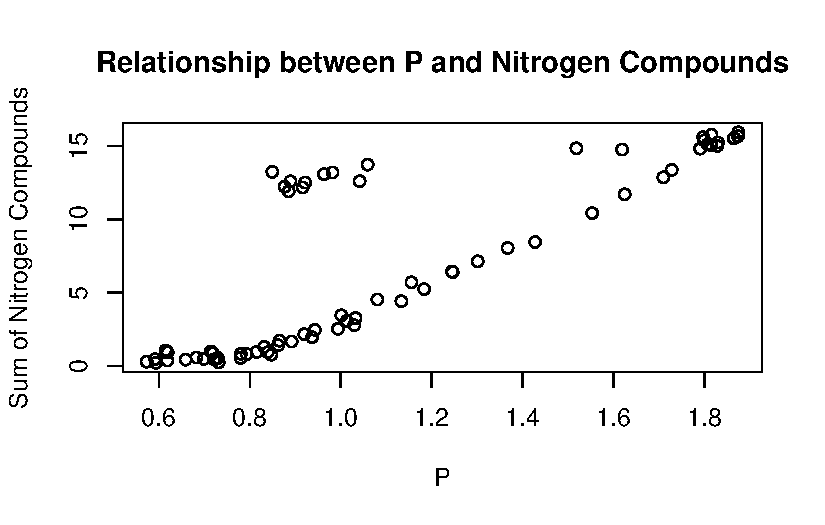
\includegraphics{Quick_Analysis_files/figure-pdf/unnamed-chunk-6-1.pdf}

\subsection{Calculations}\label{calculations}



\end{document}
